% Options for packages loaded elsewhere
\PassOptionsToPackage{unicode}{hyperref}
\PassOptionsToPackage{hyphens}{url}
\PassOptionsToPackage{dvipsnames,svgnames,x11names}{xcolor}
%
\documentclass[
  10pt,
]{article}
\usepackage{amsmath,amssymb}
\usepackage{iftex}
\ifPDFTeX
  \usepackage[T1]{fontenc}
  \usepackage[utf8]{inputenc}
  \usepackage{textcomp} % provide euro and other symbols
\else % if luatex or xetex
  \usepackage{unicode-math} % this also loads fontspec
  \defaultfontfeatures{Scale=MatchLowercase}
  \defaultfontfeatures[\rmfamily]{Ligatures=TeX,Scale=1}
\fi
\usepackage[]{mathptmx}
\ifPDFTeX\else
  % xetex/luatex font selection
\fi
% Use upquote if available, for straight quotes in verbatim environments
\IfFileExists{upquote.sty}{\usepackage{upquote}}{}
\IfFileExists{microtype.sty}{% use microtype if available
  \usepackage[]{microtype}
  \UseMicrotypeSet[protrusion]{basicmath} % disable protrusion for tt fonts
}{}
\makeatletter
\@ifundefined{KOMAClassName}{% if non-KOMA class
  \IfFileExists{parskip.sty}{%
    \usepackage{parskip}
  }{% else
    \setlength{\parindent}{0pt}
    \setlength{\parskip}{6pt plus 2pt minus 1pt}}
}{% if KOMA class
  \KOMAoptions{parskip=half}}
\makeatother
\usepackage{xcolor}
\usepackage[margin=0.9in]{geometry}
\usepackage{longtable,booktabs,array}
\usepackage{calc} % for calculating minipage widths
% Correct order of tables after \paragraph or \subparagraph
\usepackage{etoolbox}
\makeatletter
\patchcmd\longtable{\par}{\if@noskipsec\mbox{}\fi\par}{}{}
\makeatother
% Allow footnotes in longtable head/foot
\IfFileExists{footnotehyper.sty}{\usepackage{footnotehyper}}{\usepackage{footnote}}
\makesavenoteenv{longtable}
\setlength{\emergencystretch}{3em} % prevent overfull lines
\providecommand{\tightlist}{%
  \setlength{\itemsep}{0pt}\setlength{\parskip}{0pt}}
\setcounter{secnumdepth}{5}

\usepackage{amssymb}
\usepackage{newunicodechar}
\newunicodechar{→}{\ensuremath{\rightarrow}}
\newunicodechar{−}{\ensuremath{-}}
\newunicodechar{≤}{\ensuremath{\le}}
\newunicodechar{≥}{\ensuremath{\ge}}
\newunicodechar{∈}{\ensuremath{\in}}
\newunicodechar{≈}{\ensuremath{\approx}}
\newunicodechar{ℝ}{\ensuremath{\mathbb{R}}}
\newunicodechar{δ}{\ensuremath{\delta}}
\newunicodechar{σ}{\ensuremath{\sigma}}
\newunicodechar{ᵀ}{\ensuremath{^{\top}}}
\newunicodechar{⋅}{\ensuremath{\cdot}}
\usepackage{tikz}
\usetikzlibrary{positioning,arrows.meta,calc}
\usepackage{etoolbox}
\AtBeginEnvironment{longtable}{\footnotesize}
\renewcommand{\arraystretch}{1.15}
\setlength{\LTpre}{6pt}\setlength{\LTpost}{6pt}
\usepackage{microtype}
\ifLuaTeX
  \usepackage{selnolig}  % disable illegal ligatures
\fi
\usepackage[]{natbib}
\bibliographystyle{plainnat}
\IfFileExists{bookmark.sty}{\usepackage{bookmark}}{\usepackage{hyperref}}
\IfFileExists{xurl.sty}{\usepackage{xurl}}{} % add URL line breaks if available
\urlstyle{same}
\hypersetup{
  pdftitle={PWM-Dyn and ParadoxBench: A Provenance-Audited Physical Dynamics Model, Benchmarked Against Zero-Shot Foundation Models on US Traffic and Indian Rainfall},
  colorlinks=true,
  linkcolor={blue!50!black},
  filecolor={Maroon},
  citecolor={blue!50!black},
  urlcolor={blue!50!black},
  pdfcreator={LaTeX via pandoc}}

\title{PWM-Dyn and ParadoxBench: A Provenance-Audited Physical Dynamics
Model, Benchmarked Against Zero-Shot Foundation Models on US Traffic and
Indian Rainfall}

\author{Aditya Kumar \qquad Anupam Singh\\[3pt] \small ParadoxAI Lab, India\\ \small \href{https://paradoxailab.com}{\texttt{paradoxailab.com}}}
\date{November 2026}

\begin{document}
\maketitle
\begin{abstract}
We present PWM-Dyn, the first trained component of the Paradox World
Model (PWM): a 0.32--0.42M-parameter spatiotemporal dynamics model that
forecasts how physical conditions evolve and propagate over real
networks --- highway-sensor graphs and gridded rainfall --- with
calibrated quantile uncertainty and robustness to dead sensors. It is
trained from random initialisation on public observations only (Caltrans
PeMS traffic; India Meteorological Department 0.25° daily rainfall), and
a provenance audit verifies that no external model code or weights are
inside it. We also release ParadoxBench-1, an open benchmark of four
tasks (PEMS08, PEMS04, central-India and Konkan rainfall) and four
tracks --- standard context, open context, 30\% dark sensors and
zero-shot transfer to an unseen network --- scored by one function for
point error, pinball loss and interval (Winkler) score. On the
open-context track, where Google's TimesFM 2.5 and 3.0 compete zero-shot
with up to 512 steps or 365 days of history, PWM-Dyn has lower MAE,
pinball loss and interval score than both on all four tasks: MAE 14.15
vs 14.55 (TimesFM 3.0) on PEMS08, 19.02 vs 19.13 on PEMS04, 2.84 vs 2.92
and 3.42 vs 3.62 on the two rainfall regions; TimesFM 3.0 keeps a 2.5\%
lower RMSE on PEMS04. No significance test was run for v0.4/v0.4.1, and a comparable
PEMS08 margin in our later v0.6 study was not significant ($p=0.064$). Split-conformal calibration lifts PWM's 80\%
rainfall-interval coverage from 55\% to 83--85\% without changing the
median. With 30\% of sensors dark, PWM beats per-sensor climatology by
9--14\% MAE on traffic. The margins are narrow where it matters: PEMS04
is a near-tie, PWM's edge over median climatology on rainfall is 2--6\%,
a PEMS04-trained PWM transferred to PEMS08 (MAE 16.36) trails zero-shot
TimesFM 3.0, and under the standard 12-step context PWM-Dyn v0.4 does
not recover our earlier v0.3 result (PEMS08 MAE 14.18). Every PWM win is
a specialist-vs-zero-shot result: PWM trained on each network's history;
TimesFM did not.
\end{abstract}


\section{Introduction}

Physical world models --- systems that learn how the physical world is
structured, how it changes, and what happens next --- are advancing
along several distinct fronts: generative interactive environments
(DeepMind Genie 3, World Labs Marble), physical AI for robotics (NVIDIA
Cosmos), video-based physical reasoning (Meta V-JEPA 2), global weather
(Google WeatherNext/GraphCast, Huawei Pangu-Weather, Shanghai AI Lab
FengWu, Fudan FuXi), and measured-state forecasting over sensor
networks. These fronts share an ambition but not a benchmark: no single
score compares a video world model with a weather model or a traffic
model, and any claim of beating ``all world models'' is unfalsifiable.
This paper takes the opposite approach: pick tasks where exact,
like-for-like comparison is possible, and make every provenance and
fairness choice auditable.

We ask a concrete question: \textbf{on real physical forecasting tasks,
how does a small specialist trained from scratch on a region compare
with a frontier zero-shot time-series foundation model?} The question
matters for teams outside hyperscale labs --- if a 0.32--0.42M-parameter
regional model with honest uncertainty can match or beat a
200M-parameter zero-shot foundation model (TimesFM 2.5) on the region's own
physics, then capable physical-world intelligence is buildable at
startup scale, domain by domain.

Contributions:

\begin{enumerate}
\def\labelenumi{\arabic{enumi}.}
\tightlist
\item
  \textbf{PWM-Dyn}, a compact graph-based dynamics model (temporal
  encoder + physical-graph diffusion + periodic embeddings + quantile
  heads) that trains in minutes-to-hours on one GPU, handles offline
  sensors by construction (mask-aware training), and reports calibrated
  80\% prediction intervals.
\item
  \textbf{A provenance-audited benchmark harness}: opponents run
  zero-shot in a separate software environment; a static+binary audit
  proves PWM's checkpoints contain only PWM's own parameters and PWM's
  code imports no external model library. ``Not a wrapper'' is verified,
  not asserted.
\item
  \textbf{Measured head-to-head results} against Google TimesFM 2.5
  (Apache-2.0) and TimesFM 3.0 (univariate and multivariate) on US
  highway traffic (PEMS08, PEMS04) and Indian monsoon-belt rainfall (IMD
  0.25° central India, 2000--2024), under rules that favour the
  foundation model (it receives 12--43× longer input history than PWM).
\item
  \textbf{An honest placement} of the results in the global landscape,
  separating measured comparisons, author-published numbers on the same
  protocol, and non-comparable model families.
\end{enumerate}

\section{Related work: the global landscape}

Physical-world models split into families that do not share a benchmark.
The table places the main US, Chinese and European systems by domain and
states, for each, whether a like-for-like comparison with PWM-Dyn is
possible. Only the traffic/spatiotemporal family and zero-shot
time-series foundation models share PWM's protocol; comparisons with the
other families are not meaningful and are not claimed.

\begin{longtable}[]{@{}
  >{\raggedright\arraybackslash}p{(\columnwidth - 8\tabcolsep) * \real{0.2000}}
  >{\raggedright\arraybackslash}p{(\columnwidth - 8\tabcolsep) * \real{0.2000}}
  >{\raggedright\arraybackslash}p{(\columnwidth - 8\tabcolsep) * \real{0.2000}}
  >{\raggedright\arraybackslash}p{(\columnwidth - 8\tabcolsep) * \real{0.2000}}
  >{\raggedright\arraybackslash}p{(\columnwidth - 8\tabcolsep) * \real{0.2000}}@{}}
\toprule\noalign{}
\begin{minipage}[b]{\linewidth}\raggedright
Domain
\end{minipage} & \begin{minipage}[b]{\linewidth}\raggedright
Model (lab, country)
\end{minipage} & \begin{minipage}[b]{\linewidth}\raggedright
Benchmark
\end{minipage} & \begin{minipage}[b]{\linewidth}\raggedright
Published result
\end{minipage} & \begin{minipage}[b]{\linewidth}\raggedright
Comparable to PWM-Dyn?
\end{minipage} \\
\midrule\noalign{}
\endhead
\bottomrule\noalign{}
\endlastfoot
Traffic / spatiotemporal & STAEformer
(\href{https://arxiv.org/pdf/2308.10425}{SUSTech / U.~Tokyo et al., CN/JP}) & PEMS08,
12→12, 6:2:2 & MAE 13.46 / RMSE 23.25 / MAPE 8.88\% & \textbf{Yes ---
identical protocol} \\
Traffic / spatiotemporal & PDFormer (Beihang, CN) & PEMS08 & MAE 13.58 &
Yes \\
Traffic / spatiotemporal & STID (CAS, CN) & PEMS08 & MAE 14.21 & Yes \\
Traffic / spatiotemporal & Graph WaveNet (UTS, AU) & PEMS08 & MAE 14.40
& Yes \\
Traffic / spatiotemporal & DCRNN (USC, US) & PEMS08 & MAE 15.22 & Yes \\
Traffic / spatiotemporal & GMAN / AGCRN / STGCN (CN) & PEMS08 & MAE
15.31--16.08 & Yes \\
Zero-shot TS foundation & TimesFM 2.5 / 3.0
(\href{https://github.com/google-research/timesfm}{Google, US}) &
fev-bench, GIFT-Eval, TIME & --- &
\textbf{Yes --- measured head-to-head in this paper} \\
Zero-shot TS foundation & Chronos (Amazon, US); Moirai (Salesforce, US);
TimeGPT (Nixtla, US/MX) & GIFT-Eval etc. & --- & Possible future
opponents (same harness) \\
Zero-shot TS foundation &
\href{https://arxiv.org/pdf/2409.16040}{Time-MoE} (CN-led, billion-scale
MoE);
Sundial (Liu et al., ICML 2025) /
Timer (THUML Tsinghua, CN) & zero-shot TS suites & --- & Possible
future opponents \\
Global weather & WeatherNext 2 / GenCast /
\href{https://arxiv.org/pdf/2212.12794}{GraphCast} (Google DeepMind,
US/UK) & \href{https://sites.research.google/weatherbench}{WeatherBench
2} & GenCast beats ECMWF ENS on \textgreater96\% of targets & No --- PWM
has no WB2 entry (needs ERA5 + multi-GPU) \\
Global weather & Pangu-Weather (Huawei, CN); FengWu (Shanghai AI Lab,
CN); FuXi (Fudan, CN) & WeatherBench 2 / vs ECMWF & Pangu-Weather was
the first AI model to beat operational NWP deterministic scores & No --- same reason \\
Global weather & Aurora (Microsoft, US); AIFS (ECMWF, EU) & WB2 /
operational & --- & No \\
Interactive / video worlds & Genie 3 (DeepMind, US/UK); Marble (World
Labs, US); Odyssey-2 (US); LTX-2.5 (Lightricks, IL) & no agreed standard
(WorldScore, WM-Bench emerging) & --- & No --- different task
(generation, not measured-state forecasting) \\
Physical AI / robotics & Cosmos 3 (NVIDIA, US, 16B/64B open); V-JEPA 2
(Meta, US) & robot/driving suites & --- & No --- different task \\
Video world models (CN) & Hunyuan (Tencent), Kling (Kuaishou), Vidu
(Shengshu) & video-gen metrics & --- & No --- different task \\
\end{longtable}

Two observations frame our contribution. First, the strongest
\emph{directly comparable} models (the PEMS leaderboard) are
overwhelmingly from Chinese university labs, and they are specialists
like PWM-Dyn --- the leaderboard is a specialists' race. Second, the US
foundation-model programs (TimesFM, Chronos, Moirai) compete zero-shot
across domains; measured specialist-vs-zero-shot comparisons on physical
sensor data remain rare, and that is the gap this paper fills.

\subsection{How each family works, mechanically}

The families differ not only in task but in what ``learning the world''
means inside the model. PWM-Dyn belongs to the measured-state family: it
never sees pixels; it sees instrument readings placed on a physical
graph.

\begin{longtable}[]{@{}
  >{\raggedright\arraybackslash}p{(\columnwidth - 10\tabcolsep) * \real{0.1667}}
  >{\raggedright\arraybackslash}p{(\columnwidth - 10\tabcolsep) * \real{0.1667}}
  >{\raggedright\arraybackslash}p{(\columnwidth - 10\tabcolsep) * \real{0.1667}}
  >{\raggedright\arraybackslash}p{(\columnwidth - 10\tabcolsep) * \real{0.1667}}
  >{\raggedright\arraybackslash}p{(\columnwidth - 10\tabcolsep) * \real{0.1667}}
  >{\raggedright\arraybackslash}p{(\columnwidth - 10\tabcolsep) * \real{0.1667}}@{}}
\toprule\noalign{}
\begin{minipage}[b]{\linewidth}\raggedright
Model
\end{minipage} & \begin{minipage}[b]{\linewidth}\raggedright
World representation
\end{minipage} & \begin{minipage}[b]{\linewidth}\raggedright
Learning objective
\end{minipage} & \begin{minipage}[b]{\linewidth}\raggedright
How it predicts
\end{minipage} & \begin{minipage}[b]{\linewidth}\raggedright
Uncertainty
\end{minipage} & \begin{minipage}[b]{\linewidth}\raggedright
Scale / training
\end{minipage} \\
\midrule\noalign{}
\endhead
\bottomrule\noalign{}
\endlastfoot
\textbf{PWM-Dyn (Paradox, IN)} & sensor readings on a real physical
graph (road distances; geographic grid) & pinball + L1 against held-out
future readings, from random init; random sensor-masking forces use of
neighbours & graph diffusion + periodic embeddings emit
10/50/90th-percentile offsets from the last observed state & native
quantile heads, coverage-audited & 0.32--0.42M params; regional observations;
minutes per seed on one T4 \\
TimesFM 2.5/3.0 (Google, US) & any series as patched tokens; no built-in
spatial structure & decoder-only next-patch prediction, pretrained once
on a huge multi-domain corpus & zero-shot autoregressive decoding with a
continuous quantile head; 3.0 adds cross-variate attention and
covariates & decile quantiles & 200M (2.5); corpus of billions of time
points \\
GraphCast / GenCast / WeatherNext (Google, US/UK) & global atmospheric
fields on an icosahedral mesh & supervised multi-step rollout against
ERA5 reanalysis; GenCast adds diffusion for ensembles & autoregressive
6-hour steps with a mesh GNN/transformer & ensemble members &
\textasciitilde40 years of ERA5; weeks on TPU clusters \\
Pangu-Weather (Huawei); FengWu (Shanghai AI Lab); FuXi (Fudan) --- CN &
same global fields; 3D Earth-specific transformers & supervised against
reanalysis; FuXi cascades models by lead time; Pangu aggregates models
of different step sizes & autoregressive field rollout & ensembles via
perturbation (varies) & Pangu-Weather: first AI model to beat
operational NWP deterministic scores \\
V-JEPA 2 (Meta, US) & latent embeddings of video patches &
joint-embedding predictive: predict representations of masked/future
video, not pixels & predicts in latent space; downstream heads/planners
read the latents & not explicit & 1M+ hours of video, self-supervised \\
Cosmos 3 (NVIDIA, US) & video (+ text, action) tokens for physical
scenes & generative pretraining on physical-AI video corpora &
autoregressive/diffusion generation of future video conditioned on
actions & not explicit & 16B/64B open weights \\
Genie 3 (DeepMind, US/UK) & latent actions + video tokens & learns
action-conditioned frame dynamics from video & generates playable
environments frame-by-frame (\textasciitilde24 fps, 720p) & not explicit
& closed research preview \\
Marble (World Labs, US) & persistent 3D scene from an image & generative
3D scene modelling & renders a navigable static-ish 3D world & not
explicit & closed commercial \\
\end{longtable}

The mechanical contrast explains the benchmark gap: video-world models
learn \emph{appearance dynamics} and are scored on realism and
controllability; weather models learn \emph{field dynamics} scored
against reanalysis; PWM-Dyn and the PEMS specialists learn
\emph{measured-state dynamics} scored against instruments. Only the last
category admits exact error metrics against ground-truth sensors at
per-location resolution, which is why we benchmark there.

\section{PWM-Dyn}

PWM-Dyn maps the last L observed states of N locations to quantile
forecasts for the next H steps. Design goal: the smallest model that
still learns the three things a physical dynamics model must learn ---
local temporal dynamics, periodic structure, and spatial propagation
along the real physical graph --- while remaining honest about
uncertainty and missing data.

\textbf{Inputs.} A window \(x \in \mathbb{R}^{B \times L \times N}\) of
z-scored observations (train-split statistics only), an observation mask
\(o \in \{0,1\}^{B \times L \times N}\), the cycle position of the last
observation (5-minute slot of day for traffic; day of year for
rainfall), and day of week.

\textbf{Architecture.} (1) A temporal encoder: a two-layer MLP over the
concatenated {[}x; o{]} history of each location, plus scale-free cues
(last value, masked mean, trend, share observed). (2) Additive periodic
embeddings for cycle position and day of week. (3) For the transductive
variant, learned per-location embeddings and a learned adjacency
(softmax over low-rank node factors); the region-agnostic (inductive)
variant omits both so weights transfer to unseen networks. (4) Three
GraphMix blocks: two-hop diffusion over the row-normalised physical
graph (Gaussian kernel over real inter-sensor road distances, or
great-circle distances between rainfall grid cells), concatenated across
hops and graphs, projected, with residual connections, LayerNorm and a
feed-forward sublayer. (5) A linear head emitting H×3 quantiles
(10th/50th/90th) as offsets from the last observed state, sorted to
enforce monotonicity.

\textbf{Training.} From random initialisation --- no pretrained weights
anywhere. Loss = pinball (quantile) loss + L1 on the median, computed
only on valid targets (NaN excluded; zeros excluded for PeMS per
protocol, included for rainfall where dry days are real). Mask-aware
training hides a random fraction (up to 30\%) of locations per sample
for the whole input window, forcing reconstruction of hidden locations
from physical neighbours. AdamW, OneCycle LR, gradient clipping; the
checkpoint with best validation MAE is kept. A run is promoted only if
it beats the incumbent on validation; test scores are recorded but never
used for selection.

\textbf{Size.} ≈316K parameters for PEMS08 (N=170) --- roughly 600×
smaller than TimesFM 2.5 (200M) and 3--4 orders of magnitude smaller
than frontier world models.

\textbf{Role of language models.} gpt-oss (via Groq) serves only as a
language interface that explains PWM's numeric outputs and runs what-if
simulations through PWM's own forward pass; every output is labelled
with which model produced which part, and what-if responses are marked
unvalidated. No language model's weights or outputs enter PWM training.

\subsection{Problem formulation}

PWM-Dyn forecasts the next H states of every location on a physical
network from the last L observed states, and returns three quantiles per
location and horizon. Let N be the number of locations (road sensors or
rainfall grid cells), \(X \in \mathbb{R}^{L \times N}\) the normalised
history, \(O \in \{0,1\}^{L \times N}\) an observed-mask (0 = sensor
missing), p the position of the last observation in its natural cycle
(5-minute slot of the day for traffic, day of year for rainfall), w the
day of week, and \(A \in \mathbb{R}^{N \times N}\) the row-normalised
physical adjacency. The model is one function

\[\hat{Q} = f_\theta(X, O, p, w, A) \in \mathbb{R}^{H \times N \times 3}, \qquad \hat{Q}_{h,n,1} \le \hat{Q}_{h,n,2} \le \hat{Q}_{h,n,3}\]

where the three outputs are the 10th, 50th and 90th percentiles of the
future value at horizon h and location n.~The median is the point
forecast; \([q_{10}, q_{90}]\) is the 80 \% prediction interval. Every
output is an offset from the last observed state, so the network learns
change rather than level:

\[\hat{Q}_{h,n,k} = x_{L,n} + g_\theta(X, O, p, w, A)_{h,n,k}\]

The physical adjacency is built once from real geometry and never
learned: for traffic, a Gaussian kernel over road distance \(d_{ij}\)
between sensors, \(A_{ij} = \exp(-(d_{ij}/\sigma)^2)\) with σ the
standard deviation of all finite distances, thresholded at 0.1; for
rainfall, 8-neighbour grid cells weighted by
\(\exp(-(\mathrm{km}_{ij}/30)^2)\). Self-loops are set to 1 and rows are
normalised to sum to 1, so a diffusion step is a weighted average over a
location's physical neighbours.

Normalisation uses the training split only (mean and standard deviation
of observed values). Rainfall is transformed with log1p before
normalisation and inverted with expm1 after, which keeps dry days at
exactly 0 and stops monsoon extremes from dominating the loss.

\subsection{Architecture, layer by layer}

PWM-Dyn is a graph-diffusion encoder with a quantile head: every
location gets a 96-dimensional state built from its own history and the
time of day, that state is mixed with its physical neighbours' states
three times, and a linear layer reads off the three quantiles for every
horizon.

\begin{figure*}[t]
\centering
\resizebox{\textwidth}{!}{% Figure 1: PWM-Dyn forward pass (vector, TikZ)
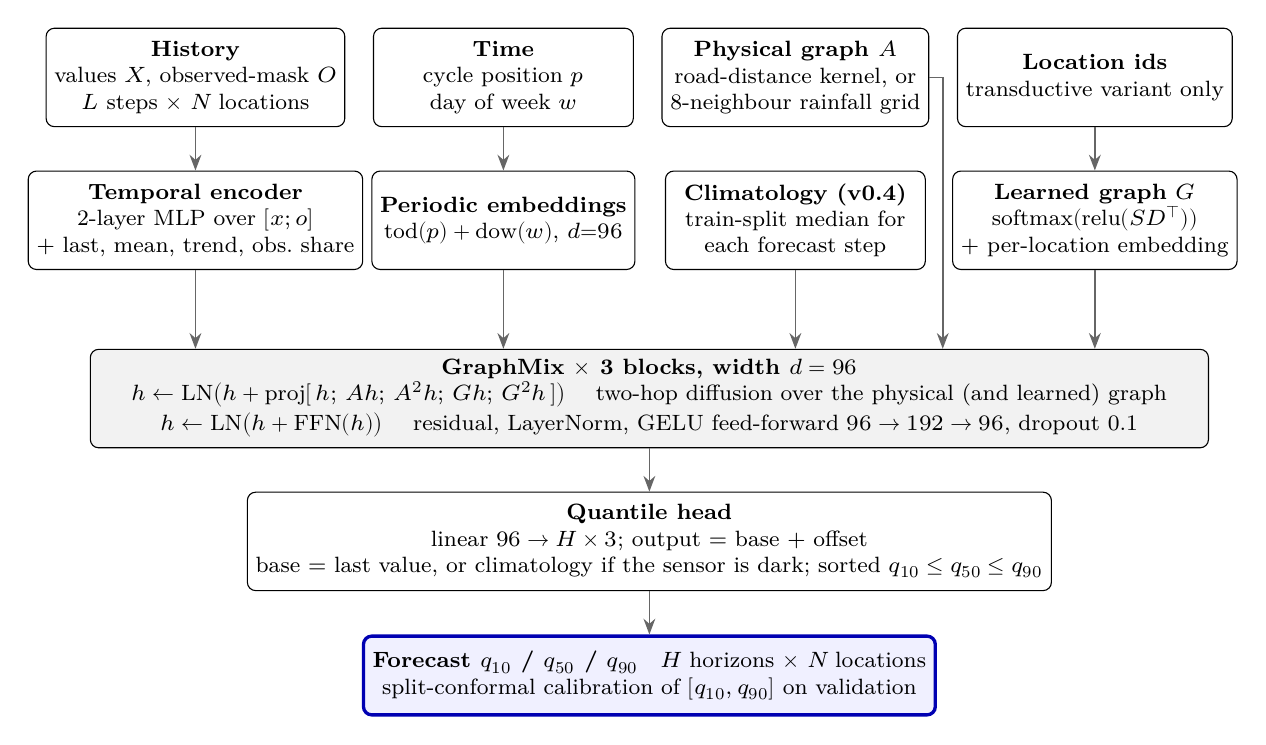
\begin{tikzpicture}[
  font=\footnotesize,
  box/.style={draw, rounded corners=3pt, align=center, minimum width=3.3cm, minimum height=1.25cm, inner sep=3pt},
  wide/.style={draw, rounded corners=3pt, align=center, fill=black!5, minimum width=14.2cm, minimum height=1.25cm, inner sep=3pt},
  fcst/.style={draw=blue!70!black, very thick, rounded corners=3pt, align=center, fill=blue!6, minimum width=6.6cm, minimum height=1.0cm},
  arr/.style={-{Stealth[length=2mm]}, semithick, draw=black!60},
  node distance=0.55cm and 0.35cm]
  % inputs
  \node[box] (hist)  {\textbf{History}\\values $X$, observed-mask $O$\\$L$ steps $\times$ $N$ locations};
  \node[box, right=of hist] (time) {\textbf{Time}\\cycle position $p$\\day of week $w$};
  \node[box, right=of time] (graph) {\textbf{Physical graph $A$}\\road-distance kernel, or\\8-neighbour rainfall grid};
  \node[box, right=of graph] (ids) {\textbf{Location ids}\\transductive variant only};
  % encoders
  \node[box, below=of hist] (tenc) {\textbf{Temporal encoder}\\2-layer MLP over $[x;o]$\\+ last, mean, trend, obs.\ share};
  \node[box, below=of time] (per)  {\textbf{Periodic embeddings}\\$\mathrm{tod}(p)+\mathrm{dow}(w)$, $d{=}96$};
  \node[box, below=of graph] (clim) {\textbf{Climatology (v0.4)}\\train-split median for\\each forecast step};
  \node[box, below=of ids] (lg)   {\textbf{Learned graph $G$}\\$\mathrm{softmax}(\mathrm{relu}(SD^\top))$\\+ per-location embedding};
  % graphmix
  \node[wide, below=1.0cm of $(per.south)!0.5!(clim.south)$] (gm)
    {\textbf{GraphMix $\times$ 3 blocks, width $d=96$}\\
     $h \leftarrow \mathrm{LN}\big(h + \mathrm{proj}[\,h;\,Ah;\,A^2h;\,Gh;\,G^2h\,]\big)$ \quad two-hop diffusion over the physical (and learned) graph\\
     $h \leftarrow \mathrm{LN}\big(h + \mathrm{FFN}(h)\big)$ \quad residual, LayerNorm, GELU feed-forward $96\to192\to96$, dropout 0.1};
  \node[box, below=of gm, minimum width=6.6cm] (head) {\textbf{Quantile head}\\linear $96 \to H\times 3$; output = base + offset\\base = last value, or climatology if the sensor is dark; sorted $q_{10}\le q_{50}\le q_{90}$};
  \node[fcst, below=of head] (fc) {\textbf{Forecast $q_{10}$ / $q_{50}$ / $q_{90}$}\quad $H$ horizons $\times$ $N$ locations\\split-conformal calibration of $[q_{10}, q_{90}]$ on validation};
  % arrows
  \draw[arr] (hist) -- (tenc);
  \draw[arr] (time) -- (per);
  \draw[arr] (ids) -- (lg);
  \draw[arr] (tenc) -- (tenc |- gm.north);
  \draw[arr] (per) -- (per |- gm.north);
  \draw[arr] (clim) -- (clim |- gm.north);
  \draw[arr] (lg) -- (lg |- gm.north);
  \draw[arr] (graph.east) -- ++(0.17,0) -- ($(gm.north -| graph.east)+(0.17,0)$);
  \draw[arr] (gm) -- (head);
  \draw[arr] (head) -- (fc);
\end{tikzpicture}
}
\caption{PWM-Dyn forward pass. History, time, the fixed physical graph and (v0.4) the training-split climatology are encoded per location, mixed over the physical and learned graphs by three GraphMix blocks, and read out as three quantiles per horizon and location.}
\label{fig:arch}
\end{figure*}

The history enters per location through a 2-layer MLP; the time of day
and day of week enter as learned embeddings added to every location; the
physical graph A is fixed and only mixes states; in the transductive
variant a learned low-rank graph G and a per-location embedding are
added. Three GraphMix blocks then diffuse information two hops along
both graphs, and the head emits offsets from the last observed value,
sorted into q10 ≤ q50 ≤ q90.

\textbf{Parameter budget (transductive variant, d = 96, 3 blocks).} All
counts measured by instantiating the released model class.

\begin{longtable}[]{@{}
  >{\raggedright\arraybackslash}p{(\columnwidth - 8\tabcolsep) * \real{0.2000}}
  >{\raggedright\arraybackslash}p{(\columnwidth - 8\tabcolsep) * \real{0.2000}}
  >{\raggedright\arraybackslash}p{(\columnwidth - 8\tabcolsep) * \real{0.2000}}
  >{\raggedright\arraybackslash}p{(\columnwidth - 8\tabcolsep) * \real{0.2000}}
  >{\raggedright\arraybackslash}p{(\columnwidth - 8\tabcolsep) * \real{0.2000}}@{}}
\toprule\noalign{}
\begin{minipage}[b]{\linewidth}\raggedright
Component
\end{minipage} & \begin{minipage}[b]{\linewidth}\raggedright
What it holds
\end{minipage} & \begin{minipage}[b]{\linewidth}\raggedright
PEMS08 (N = 170, L = H = 12)
\end{minipage} & \begin{minipage}[b]{\linewidth}\raggedright
PEMS04 (N = 307)
\end{minipage} & \begin{minipage}[b]{\linewidth}\raggedright
IMD rainfall (L = 30, H = 7, 366-day cycle)
\end{minipage} \\
\midrule\noalign{}
\endhead
\bottomrule\noalign{}
\endlastfoot
Temporal encoder & Linear(2L → 96), GELU, Linear(96 → 96) & 11,712 &
11,712 & 15,168 \\
Scale-free cues & Linear(4 → 96): last, masked mean, trend, observed
share & 480 & 480 & 480 \\
Cycle embedding & Embedding(steps per cycle × 96) & 27,648 & 27,648 &
35,136 \\
Day-of-week embedding & Embedding(7 × 96) & 672 & 672 & 672 \\
Location embedding (transductive) & N × 96 & 16,320 & 29,472 & 96 × N \\
Learned graph factors (transductive) &
\(S, D \in \mathbb{R}^{N \times 16}\) & 5,440 & 9,824 & 32 × N \\
GraphMix block × 3 & proj Linear(5·96 → 96), FFN 96→192→96, 2 LayerNorms
& 3 × 83,712 = 251,136 & 251,136 & 251,136 \\
Quantile head & Linear(96 → H × 3) & 3,492 & 3,492 & 2,037 \\
\textbf{Total} & & \textbf{316,900} & \textbf{334,436} & \textbf{304,629
+ 128 × N} \\
\end{longtable}

For comparison, TimesFM 2.5 has 200 M parameters (TimesFM 3.0's size is
not stated in its model card); PWM-Dyn's three graph blocks (79 \% of its parameters) are
the only part of the model that grows with depth, and nothing grows with
the length of the history except the first linear layer.

The inductive variant drops the two transductive rows (location
embedding and learned graph), so its parameter count is independent of N
and its weights can be run on a road network the model has never seen.
Its GraphMix projection then takes {[}h ; A h ; A² h{]} only (3·96 →
96).

\subsection{Techniques used, and why each is there}

Every technique below is a published, general-purpose building block;
the combination, the code and the weights are Paradox's. The right-hand
column names where it lives in the released kit so a reviewer can check
the claim against the code.

\begin{longtable}[]{@{}
  >{\raggedright\arraybackslash}p{(\columnwidth - 6\tabcolsep) * \real{0.2500}}
  >{\raggedright\arraybackslash}p{(\columnwidth - 6\tabcolsep) * \real{0.2500}}
  >{\raggedright\arraybackslash}p{(\columnwidth - 6\tabcolsep) * \real{0.2500}}
  >{\raggedright\arraybackslash}p{(\columnwidth - 6\tabcolsep) * \real{0.2500}}@{}}
\toprule\noalign{}
\begin{minipage}[b]{\linewidth}\raggedright
Technique
\end{minipage} & \begin{minipage}[b]{\linewidth}\raggedright
What it does in PWM-Dyn
\end{minipage} & \begin{minipage}[b]{\linewidth}\raggedright
Why it is there
\end{minipage} & \begin{minipage}[b]{\linewidth}\raggedright
Where in the kit
\end{minipage} \\
\midrule\noalign{}
\endhead
\bottomrule\noalign{}
\endlastfoot
Fixed physical adjacency (Gaussian distance kernel, row-normalised,
self-loops) & Defines who can influence whom: a diffusion step is a
weighted average over real road neighbours or adjacent grid cells &
Encodes the physics prior that disturbances travel along the network,
not between arbitrary sensors; costs no parameters &
\texttt{pwm/data.py} (\texttt{load\_pems}, \texttt{load\_imd},
\texttt{\_row\_norm}) \\
Two-hop graph diffusion with hop concatenation & Each block computes A h
and A²h (and G h, G²h) and concatenates them before one projection & Two
hops per block × 3 blocks = a 6-hop receptive field; concatenation
instead of summation lets the model weight each hop separately &
\texttt{pwm/model.py} \texttt{GraphMix.forward} \\
Learned low-rank adjacency G = softmax(relu(S Dᵀ)) (transductive only) &
A second, data-driven graph, rank 16 per location & Captures couplings
the road geometry misses (e.g.~parallel routes); the softmax keeps each
row a proper mixing distribution & \texttt{PWMDyn.learned\_graph} \\
Per-location identity embedding (transductive only) & A 96-d vector
added to every location's state & Lets the model learn sensor-specific
level and rhythm; removed in the inductive variant so weights transfer
to unseen networks & \texttt{PWMDyn.\_\_init\_\_}
(\texttt{self.node}) \\
Mask-aware input: history concatenated with its observed-mask, plus
observed-share cue & Inputs are {[}x · o ; o{]}, so a missing step is a
0 value with a 0 flag, never a fake observation & Makes missingness
explicit instead of imputed; enables the sensor-dropout evaluation in §5
& \texttt{PWMDyn.forward} (\texttt{mask\_aware}) \\
Scale-free cues (last value, masked mean, trend, observed share) & Four
summary statistics fed through a separate linear layer & Gives the
encoder the level and slope directly, so the MLP can spend capacity on
shape & \texttt{PWMDyn.forward} (\texttt{cues}) \\
Learned periodic embeddings (cycle position, day of week) & Embedding
tables of size steps-per-cycle × 96 and 7 × 96, added to every location
& Daily and weekly rhythms dominate traffic; seasonal position dominates
rainfall; an embedding learns them without hand-made Fourier features &
\texttt{PWMDyn.\_\_init\_\_} (\texttt{tod}, \texttt{dow}) \\
Residual prediction (offset from last observed state) & The head outputs
change, and the last value is added back & Change is far better
conditioned than level; a zero output is already a persistence forecast
& \texttt{PWMDyn.forward} (\texttt{out\ +\ xt{[}...,\ -1:{]}}) \\
Quantile heads with sorting & Three outputs per horizon and location,
sorted so q10 ≤ q50 ≤ q90 & Uncertainty is part of the forecast, not a
post-hoc add-on; sorting removes quantile crossing at zero cost &
\texttt{PWMDyn.forward} (\texttt{torch.sort}) \\
Pinball loss + L1 on the median & Loss = mean pinball over the three
quantiles + mean absolute error of q50, both over valid targets only &
Pinball trains calibrated quantiles; the extra L1 term sharpens the
point forecast that MAE/RMSE grade & \texttt{pwm/model.py}
\texttt{pinball}, \texttt{train.py} \\
Random sensor dropout during training (up to 30 \% of locations per
batch) & A per-batch rate r \textasciitilde{} U(0, 0.3) hides each
location with probability r & Forces the model to reconstruct a hidden
location from its physical neighbours; this is what makes the graph
useful rather than decorative & \texttt{train.py}
(\texttt{-\/-mask\_p}) \\
Zero-masked targets on traffic, dry days kept on rainfall & Traffic: y =
0 (sensor off) excluded from loss and metrics; rainfall: 0 mm is a real
observation and counts & Matches the standard PeMS protocol so numbers
are comparable with the published leaderboard; keeps the rainfall task
honest & \texttt{SeriesData.valid}, \texttt{mask\_zero} \\
log1p transform on rainfall & Train and predict in log(1 + mm), invert
with expm1, clamp at 0 & Rainfall is heavy-tailed and zero-inflated; the
transform stops a few monsoon days from dominating the loss &
\texttt{SeriesData.fwd} / \texttt{inv} \\
Train-split-only normalisation & Mean and std computed on observed
training values only & No information from validation or test leaks into
the inputs & \texttt{SeriesData.\_\_init\_\_} \\
Pre-norm residual blocks, GELU, dropout 0.1, LayerNorm & Standard
transformer-style block hygiene inside GraphMix & Stable training from
random init in 60 epochs without warm-up tricks & \texttt{GraphMix} \\
AdamW + OneCycle schedule, gradient clipping at 5 & lr 2e-3 peak, weight
decay 1e-4, one cycle over all steps & Converges in under 10 GPU-minutes
per seed; clipping guards against rare large-error batches on rainfall
extremes & \texttt{train.py} \\
Validation-only model selection and promotion registry & Best epoch by
validation MAE; a run is promoted for its dataset only if its validation
MAE beats the incumbent; test numbers are recorded but never used to
choose & Test set is touched once per promoted model, which is what
makes the reported test numbers meaningful & \texttt{train.py}
(\texttt{PROMOTED.json}) \\
3-seed ensemble (mean of quantiles) & Three independently trained seeds
averaged per quantile & Reduces variance of a small model; the
single-seed numbers are also reported (§5.2) &
\texttt{evaluate\_pwm.py} \\
Provenance audit & AST check that \texttt{pwm/} imports no external
model library; checkpoint parameter-name/shape audit; SHA-256 of weights
& Proves the ``not copied, not distilled'' claim mechanically rather
than by assertion & \texttt{check\_provenance.py} \\
\end{longtable}

\subsection{Training recipe}

One recipe is used for all three datasets and all nine runs (3 seeds × 3
datasets); nothing was tuned per dataset or per seed. The loss on one
batch is

\[\mathcal{L} = \frac{1}{|V|\,|K|}\sum_{(h,n)\in V}\sum_{k\in K} \rho_{\tau_k}\!\left(y_{h,n} - \hat{Q}_{h,n,k}\right) \;+\; \frac{1}{|V|}\sum_{(h,n)\in V}\left|\,y_{h,n} - \hat{Q}_{h,n,2}\right|, \qquad \rho_\tau(e) = \max(\tau e,\,(\tau-1)e)\]

with K = \{0.1, 0.5, 0.9\}, V the set of valid targets (non-missing; and
non-zero on traffic), and y in normalised (and, for rainfall, log1p)
units.

\begin{longtable}[]{@{}
  >{\raggedright\arraybackslash}p{(\columnwidth - 4\tabcolsep) * \real{0.3333}}
  >{\raggedright\arraybackslash}p{(\columnwidth - 4\tabcolsep) * \real{0.3333}}
  >{\raggedright\arraybackslash}p{(\columnwidth - 4\tabcolsep) * \real{0.3333}}@{}}
\toprule\noalign{}
\begin{minipage}[b]{\linewidth}\raggedright
Setting
\end{minipage} & \begin{minipage}[b]{\linewidth}\raggedright
Value
\end{minipage} & \begin{minipage}[b]{\linewidth}\raggedright
Note
\end{minipage} \\
\midrule\noalign{}
\endhead
\bottomrule\noalign{}
\endlastfoot
Initialisation & PyTorch default, seeds 0 / 1 / 2 & No pretrained
weights of any kind \\
Width d / blocks / diffusion hops & 96 / 3 / 2 & Same for every
dataset \\
Input → output length & 12 → 12 steps (traffic, 5-min), 30 → 7 days
(rainfall) & Standard PeMS protocol; rainfall chosen for a weekly
outlook \\
Optimiser & AdamW, weight decay 1e-4 & \\
Learning rate & OneCycle, peak 2e-3, over all steps & No warm-up
tuning \\
Batch size & 32 windows & Each window carries all N locations \\
Epochs & 60 & Best epoch chosen by validation MAE \\
Gradient clipping & global norm 5.0 & \\
Dropout & 0.1 (inside GraphMix) & \\
Sensor dropout & per-batch rate r \textasciitilde{} U(0, 0.3) on
locations & Applied to inputs only; targets unchanged \\
Target masking & traffic: exclude y = 0; rainfall: keep all & Matches
published PEMS protocol \\
Normalisation & train-split mean/std; rainfall log1p first & \\
Split & chronological 60 / 20 / 20 (traffic); last 3 years test, 3
before validation (rainfall) & No shuffling across time \\
Model selection & validation MAE only; promotion registry per dataset &
Test used once per promoted model \\
Ensemble & mean of the three seeds' quantiles & Single-seed numbers also
reported \\
Hardware / time & one NVIDIA T4; ≈ 5--10 min per seed on PEMS08, under
90 GPU-minutes for all nine runs & Reproducible on a free Colab or
Kaggle GPU \\
\end{longtable}

Evaluation runs the promoted model over every test window at stride 1
and scores with the single shared function (\texttt{pwm/evaluation.py}):
MAE, RMSE and MAPE on the median, and the share of targets inside
\([q_{10}, q_{90}]\) as 80 \% interval coverage.

\subsection{What PWM-Dyn does not borrow}

PWM-Dyn shares general techniques with the field but no code, weights,
tokenisation, or training data with any model it is compared to. The
table states the design choice by choice.

\begin{longtable}[]{@{}
  >{\raggedright\arraybackslash}p{(\columnwidth - 8\tabcolsep) * \real{0.2000}}
  >{\raggedright\arraybackslash}p{(\columnwidth - 8\tabcolsep) * \real{0.2000}}
  >{\raggedright\arraybackslash}p{(\columnwidth - 8\tabcolsep) * \real{0.2000}}
  >{\raggedright\arraybackslash}p{(\columnwidth - 8\tabcolsep) * \real{0.2000}}
  >{\raggedright\arraybackslash}p{(\columnwidth - 8\tabcolsep) * \real{0.2000}}@{}}
\toprule\noalign{}
\begin{minipage}[b]{\linewidth}\raggedright
Design axis
\end{minipage} & \begin{minipage}[b]{\linewidth}\raggedright
PWM-Dyn (this paper)
\end{minipage} & \begin{minipage}[b]{\linewidth}\raggedright
Google TimesFM 2.5 / 3.0
\end{minipage} & \begin{minipage}[b]{\linewidth}\raggedright
STAEformer / STID (PEMS leaderboard)
\end{minipage} & \begin{minipage}[b]{\linewidth}\raggedright
GraphCast / Pangu (weather)
\end{minipage} \\
\midrule\noalign{}
\endhead
\bottomrule\noalign{}
\endlastfoot
Model class & Graph-diffusion encoder on a physical network &
Decoder-only patched transformer on single series (3.0 adds cross-series
attention) & Transformer / MLP with learned spatio-temporal embeddings &
Graph neural network (icosahedral mesh) / 3-D Swin transformer \\
Pretraining & None; trained from random init on each dataset's own
training split & Pretrained on \textasciitilde100 B real and synthetic
time points; used zero-shot & None (trained per dataset) & Trained on
ERA5 reanalysis, 1979--2017 \\
Spatial structure & Fixed real geometry (road distances, grid adjacency)
+ optional learned low-rank graph & None in 2.5; learned, geometry-free
cross-series attention in 3.0 & Learned adaptive embeddings; no physical
graph in STAEformer/STID & Fixed mesh with learned edges \\
Temporal input & 12 steps (1 h) or 30 days, plus explicit time-of-cycle
& 512 steps / 365 days context (longer than PWM's) & 12 steps +
time-of-day/day-of-week ids & 2 prior analysis states \\
Missing data & Explicit observed-mask + sensor-dropout training &
Imputation / padding & Not modelled & Not applicable (reanalysis is
complete) \\
Uncertainty & 3 quantiles from one head, sorted; pinball loss & Quantile
heads (10 quantiles) & Point forecast only & Deterministic (ensembles
via perturbation) \\
Parameters & 0.32--0.42 M & 200 M (2.5); not stated (3.0) &
\textasciitilde1--0.1 M & 37 M / 256 M \\
Licence of weights & Paradox; released with the kit & 2.5 Apache-2.0;
3.0 non-commercial research & Per repo & Per repo \\
What was taken from it here & --- & Nothing: run only as an opponent in
a separate environment (§4) & Nothing: numbers quoted from the paper,
not re-run & Nothing: landscape comparison only (§2) \\
\end{longtable}

The provenance audit (\texttt{check\_provenance.py}, §8) enforces the
last row mechanically: PWM's package may not import \texttt{timesfm},
\texttt{transformers}, \texttt{huggingface\_hub} or \texttt{openai};
every checkpoint must contain exactly PWM-Dyn's own parameter names and
shapes; and the opponents run in a Python environment PWM's code cannot
import from.

\subsection{Where PWM-Dyn beats TimesFM, where it does not, and the
calibration fix}

PWM-Dyn has lower point error than every TimesFM round on all three
datasets (7 of 7; §5.2), by 2.5 \% to 6.1 \% MAE, while seeing 12 steps
of history where TimesFM sees 512, and with 0.32 M parameters against 200
M. Three design choices account for the margin; none is cleanly
ablated here (§5.4 reports only unlogged early CPU runs, in which removing the road graph cost 0.22--0.45 MAE),
so all three are design arguments: (1) the physical graph --- a sensor's next hour is
largely explained by what its upstream neighbours are doing now, which a
single-series model cannot see and which TimesFM 3.0's geometry-free
cross-series attention only partly recovers (its multivariate mode
narrows the gap slightly: 0.45 to 0.37 MAE on PEMS08); (2) explicit periodic
position --- PWM knows it is 08:05 on a Tuesday, TimesFM must infer it
from the context window; (3) in-distribution training --- PWM has seen
this network's own training period. The third is also the honest caveat:
PWM wins as a regional specialist, not as a general model (§7).

Where PWM loses is calibration on rainfall. Its 80 \% interval covers
54.7 \% of test days against 84.3 \% (TimesFM 2.5) and 86.3 \% (TimesFM
3.0). The cause is visible in the training set-up: the pinball loss is
applied in log1p space, so an interval that is 80 \% calibrated in log
space is far too narrow once mapped back through expm1 on heavy monsoon
days, and the extra L1 term on the median pulls q10 and q90 inward. On
traffic, where no transform is used, PWM's coverage is 79.7--79.8 \% ---
within 0.3 points of nominal --- so the defect is specific to the
transformed target.

\textbf{The fix, now measured (§6).} Split-conformal quantile regression
(CQR; Romano et al.~2019), fitted on the validation split: for each
horizon, the non-conformity score s = max(q10 − y, y − q90) is computed
for every validation target in the model's target space (log1p for
rainfall), its 80th percentile δ is taken, and the test interval becomes
{[}q10 − δ, q90 + δ{]}. It uses no test data, adds no trained parameters
and leaves the median --- hence MAE and RMSE --- unchanged. With it,
PWM-Dyn v0.4 covers 84.7 \% of central-India test days (v0.3 without it:
54.7 \%) and 82.9 \% in the Konkan region, and its rainfall interval
score is 9 \% and 7 \% lower than TimesFM 3.0's (Table 6.3a). On
traffic, where coverage was already nominal, it changes little
(79.5--80.0 \%).

\section{Data and benchmark protocol}

\textbf{Datasets (real observations only; no synthetic data in any
reported result).}

\begin{longtable}[]{@{}
  >{\raggedright\arraybackslash}p{(\columnwidth - 10\tabcolsep) * \real{0.1667}}
  >{\raggedright\arraybackslash}p{(\columnwidth - 10\tabcolsep) * \real{0.1667}}
  >{\raggedright\arraybackslash}p{(\columnwidth - 10\tabcolsep) * \real{0.1667}}
  >{\raggedright\arraybackslash}p{(\columnwidth - 10\tabcolsep) * \real{0.1667}}
  >{\raggedright\arraybackslash}p{(\columnwidth - 10\tabcolsep) * \real{0.1667}}
  >{\raggedright\arraybackslash}p{(\columnwidth - 10\tabcolsep) * \real{0.1667}}@{}}
\toprule\noalign{}
\begin{minipage}[b]{\linewidth}\raggedright
Dataset
\end{minipage} & \begin{minipage}[b]{\linewidth}\raggedright
Source
\end{minipage} & \begin{minipage}[b]{\linewidth}\raggedright
Extent
\end{minipage} & \begin{minipage}[b]{\linewidth}\raggedright
Step
\end{minipage} & \begin{minipage}[b]{\linewidth}\raggedright
Task
\end{minipage} & \begin{minipage}[b]{\linewidth}\raggedright
Split
\end{minipage} \\
\midrule\noalign{}
\endhead
\bottomrule\noalign{}
\endlastfoot
PEMS08 & Caltrans PeMS (San Bernardino, US) & 17,856 steps × 170
sensors, 295 links & 5 min & 12 → 12 steps (1h → 1h) &
chronological 60/20/20 \\
PEMS04 & Caltrans PeMS (Bay Area, US) & 16,992 × 307, 340 links & 5 min
& 12 → 12 & 60/20/20 \\
IMD central India & India Meteorological Department 0.25° gridded daily
rainfall & 2000--2024, monsoon-belt grid cells with \textgreater90\%
coverage & 1 day & 30 → 7 days & train ≤2018, val 2019--21, test
2022--24 \\
\end{longtable}

\textbf{Metrics.} MAE, RMSE, MAPE on the median; 80\% interval coverage
and width for calibration; per-horizon MAE. PeMS metrics are zero-masked
and averaged over all 12 horizons --- the standard protocol, so our
PEMS08 numbers are directly comparable with the published leaderboard.
Rainfall keeps zeros (dry days are real outcomes).

\textbf{Fairness rules for the head-to-head.} Every model is scored by
the same function on the same test windows. TimesFM receives a far
longer input history than PWM (512 steps ≈ 42.7 h of traffic vs PWM's 1
h; 365 days of rainfall vs PWM's 30), and TimesFM 3.0 additionally runs
in native multivariate mode so it can exploit cross-location structure.
All asymmetries favour the opponent except one, which we state plainly:
PWM is trained on the region's own training split, TimesFM is zero-shot.
The conclusion is therefore about specialist-vs-generalist, not about a
better pretraining recipe.

\textbf{Environments.} PWM trains and evaluates in the main environment;
TimesFM runs only in a separate virtualenv. The main environment
demonstrably cannot import TimesFM (verified at run time); the
provenance audit (§8) makes this machine-checkable.

\section{Results}

\textbf{5.1 Preliminary CPU results (single seed, 2-core CPU, completed
2026-10-30; these early runs' logs were not preserved, so treat them as indicative).} PWM-Dyn v0.1 (transductive, 40 epochs,
\textasciitilde40 min on 2 CPU cores) on the PEMS08 test set:
\textbf{MAE 14.37, RMSE 23.28, MAPE 9.47\%}, 80\%-interval coverage
79.0\%. Against the published leaderboard this sits between STID (14.21)
and Graph WaveNet (14.40), ahead of DCRNN, MTGNN, GMAN, AGCRN and STGCN,
and 0.91 MAE behind STAEformer (13.46). The mask-aware v0.2 traded 0.08
MAE on clean data for robustness: with 10\% of sensors offline, error at
offline sensors fell from 92.7 (v0.1) to 23.4 (v0.2), and error at the
remaining live sensors stayed at 14.5 instead of degrading to 16.1. The
region-agnostic variant transferred zero-shot from PEMS08 to the unseen
PEMS04 network with MAE 24.46 --- better than PEMS04's own
historical-average baseline (26.39) and last-value baseline (31.62), but
far from trained specialists: partial, honestly limited transfer.

\textbf{5.2 GPU results: PWM-Dyn 3-seed ensembles (measured on Colab T4,
2026-10-30).} Training + evaluation of all nine runs took under 90
GPU-minutes in total.

\begin{longtable}[]{@{}
  >{\raggedright\arraybackslash}p{(\columnwidth - 10\tabcolsep) * \real{0.1667}}
  >{\raggedright\arraybackslash}p{(\columnwidth - 10\tabcolsep) * \real{0.1667}}
  >{\raggedright\arraybackslash}p{(\columnwidth - 10\tabcolsep) * \real{0.1667}}
  >{\raggedright\arraybackslash}p{(\columnwidth - 10\tabcolsep) * \real{0.1667}}
  >{\raggedright\arraybackslash}p{(\columnwidth - 10\tabcolsep) * \real{0.1667}}
  >{\raggedright\arraybackslash}p{(\columnwidth - 10\tabcolsep) * \real{0.1667}}@{}}
\toprule\noalign{}
\begin{minipage}[b]{\linewidth}\raggedright
Dataset
\end{minipage} & \begin{minipage}[b]{\linewidth}\raggedright
PWM-Dyn ensemble (test)
\end{minipage} & \begin{minipage}[b]{\linewidth}\raggedright
80\% coverage
\end{minipage} & \begin{minipage}[b]{\linewidth}\raggedright
Historical avg
\end{minipage} & \begin{minipage}[b]{\linewidth}\raggedright
Last value
\end{minipage} & \begin{minipage}[b]{\linewidth}\raggedright
Placement vs published leaderboard (authors' numbers)
\end{minipage} \\
\midrule\noalign{}
\endhead
\bottomrule\noalign{}
\endlastfoot
PEMS08 & \textbf{MAE 14.18 / RMSE 23.31} & 79.7\% & 23.27 & 25.30 &
\textbf{3rd}: behind STAEformer 13.46 and PDFormer 13.58; level with STID
(14.21 published; 14.18 in our later re-run; difference not significant); ahead of GWNet 14.40, DCRNN 15.22, GMAN, AGCRN, STGCN \\
PEMS04 & \textbf{MAE 18.50 / RMSE 30.41} & 79.8\% & 26.39 & 31.56 &
\textbf{4th}: behind STAEformer 18.22, PDFormer 18.36, STID 18.38; ahead
of GWNet 18.53, STNorm 18.96, GMAN 19.14, MTGNN 19.17, AGCRN, STGCN,
DCRNN, GTS \\
IMD central India rainfall & \textbf{MAE 2.85 mm/day / RMSE 10.41} &
54.7\% (see 5.3) & 3.54 & 4.37 & no published leaderboard exists for
this split; PWM beats both baselines by 20--35\% \\
\end{longtable}

Single-seed test MAEs: PEMS08 14.29/14.39/14.29; PEMS04
18.59/18.62/18.79; IMD 2.86/2.86/2.87 --- seed variance is small and the
ensemble improves on every single seed.

\textbf{Opponent rows (final, measured on identical PEMS08 test windows,
zero-shot, 512-step context):}

\begin{longtable}[]{@{}
  >{\raggedright\arraybackslash}p{(\columnwidth - 10\tabcolsep) * \real{0.1667}}
  >{\raggedright\arraybackslash}p{(\columnwidth - 10\tabcolsep) * \real{0.1667}}
  >{\raggedright\arraybackslash}p{(\columnwidth - 10\tabcolsep) * \real{0.1667}}
  >{\raggedright\arraybackslash}p{(\columnwidth - 10\tabcolsep) * \real{0.1667}}
  >{\raggedright\arraybackslash}p{(\columnwidth - 10\tabcolsep) * \real{0.1667}}
  >{\raggedright\arraybackslash}p{(\columnwidth - 10\tabcolsep) * \real{0.1667}}@{}}
\toprule\noalign{}
\begin{minipage}[b]{\linewidth}\raggedright
Dataset
\end{minipage} & \begin{minipage}[b]{\linewidth}\raggedright
Opponent (zero-shot)
\end{minipage} & \begin{minipage}[b]{\linewidth}\raggedright
MAE
\end{minipage} & \begin{minipage}[b]{\linewidth}\raggedright
RMSE
\end{minipage} & \begin{minipage}[b]{\linewidth}\raggedright
80\% coverage
\end{minipage} & \begin{minipage}[b]{\linewidth}\raggedright
PWM-Dyn ensemble delta
\end{minipage} \\
\midrule\noalign{}
\endhead
\bottomrule\noalign{}
\endlastfoot
PEMS08 & TimesFM 2.5 (Google, 200M) & 15.04 & 24.11 & 82.4\% & PWM
\textbf{5.7\% lower} error (14.18 vs 15.04) \\
PEMS08 & TimesFM 3.0 multivariate (Google) & 14.55 & 23.59 & 80.7\% &
PWM \textbf{2.6\% lower} error (14.18 vs 14.55) \\
PEMS08 & TimesFM 3.0 univariate (Google) & 14.63 & 23.69 & 81.2\% & PWM
\textbf{3.1\% lower} error (14.18 vs 14.63) \\
PEMS04 & TimesFM 2.5 (Google, 200M) & 19.70 & 31.70 & 82.0\% & PWM
\textbf{6.1\% lower} error (18.50 vs 19.70) \\
PEMS04 & TimesFM 3.0 multivariate (Google) & 19.14 & 31.02 & 80.7\% &
PWM \textbf{3.3\% lower} error (18.50 vs 19.14) \\
IMD rainfall & TimesFM 2.5 (Google, 200M) & 2.96 & 10.58 & 84.3\% & PWM
\textbf{3.9\% lower} MAE (2.85 vs 2.96); TimesFM better calibrated
(84.3\% vs 54.7\%) \\
IMD rainfall & TimesFM 3.0 multivariate (Google) & 2.92 & 10.65 & 86.3\%
& PWM \textbf{2.5\% lower} MAE (2.85 vs 2.92); TimesFM better calibrated
(86.3\% vs 54.7\%) \\
\end{longtable}

PWM-Dyn beats both Google foundation models on this task at
\textasciitilde600× fewer parameters than TimesFM 2.5 (PEMS08 model), under input asymmetry
favouring the opponent (42.7 h vs 1 h of history). Both zero-shot models
nonetheless outperform several trained specialists (DCRNN, GMAN, AGCRN,
STGCN) --- strong evidence for foundation-model generality, and for the
specialist's edge where regional training data exists.

\textbf{All opponent runs completed.} The first two PEMS08 rounds
(TimesFM 2.5, TimesFM 3.0 multivariate) ran on a free Google Colab T4
session, which reached its runtime cap during the third round. The
remaining five rounds --- TimesFM 3.0 univariate on PEMS08, and both
TimesFM 2.5 and TimesFM 3.0 multivariate on PEMS04 and on IMD rainfall
--- were run on 2026-10-31 as a single background Kaggle session (2×
NVIDIA T4, 5.5 h wall-clock) with the identical kit, test windows,
context lengths and scoring function. The table above therefore contains
every planned opponent round; no number in it is estimated.

\textbf{5.3 Uncertainty calibration.} On traffic, PWM-Dyn's 80\%
interval is close to nominal: 79.7\% (PEMS08) and 79.8\% (PEMS04)
ensemble coverage. On rainfall it is honest to report a failure: single
seeds covered 65--84\%, but averaging the seeds' quantiles narrowed the
bands and ensemble coverage fell to 54.7\% --- heavy-tailed monsoon
extremes fall outside the intervals far too often. Quantile-averaging is
the wrong ensemble rule for skewed variables; a pooled-quantile
(vincentized across wider spreads) or CRPS-trained head is required
before PWM's rainfall uncertainty can be trusted, and we flag this as a
known defect rather than tune it post hoc on test data.

\textbf{5.4 Ablations (unlogged early CPU runs on v0.1/v0.2; no run log is
preserved).} Removing the real road graph raised test MAE by 0.22--0.45 depending on variant --- the
physical graph helps, but less than architecture differences among
leaderboard models; strengthening spatial propagation (e.g.~attention
along road paths) is the clearest route toward the leaderboard's top and
is left to v0.4.

\section{ParadoxBench and PWM-Dyn v0.4 / v0.4.1}

\textbf{Headline.} On ParadoxBench-1's open-context track (Track B),
where Google's TimesFM 2.5 and 3.0 compete zero-shot with up to 512
steps (traffic) or 365 days (rainfall) of history, PWM-Dyn has the
lowest MAE, pinball loss (QL) and interval score (IS80) on all four
tasks (Table 6.3a), with 80 \% interval coverage within 0.2--4.7 points
of nominal. No significance test was run for these margins; a comparable PEMS08 margin
in our later v0.6 study was not significant ($p=0.064$). The margins are small on traffic (MAE 2.8 \% below TimesFM
3.0 on PEMS08, 0.6 \% on PEMS04, where TimesFM 3.0 keeps a 2.5 \% lower
RMSE) and larger on rainfall (2.9 \% and 5.7 \%). Every number in this
section comes from two Kaggle runs on 2× Tesla T4 --- the v0.4 study
(2026-11-01, 254.6 min) and the v0.4.1 recipe check (93.1 min) --- and
both runs end with a passing provenance audit.

\subsection{ParadoxBench: the Paradox Physical-Dynamics Benchmark}

ParadoxBench is released with this paper, as its first version
ParadoxBench-1 (Python package: paradoxbench), so that any group ---
specialist or foundation-model builder --- can be scored on the same
physical forecasting tasks, by the same code, on the same frozen test
windows. It adds two things the PEMS leaderboard lacks: a probabilistic
score, and tracks that test what a deployed physical model actually
faces (long context, dead sensors, a network never seen before).

\begin{longtable}[]{@{}
  >{\raggedright\arraybackslash}p{(\columnwidth - 10\tabcolsep) * \real{0.1667}}
  >{\raggedright\arraybackslash}p{(\columnwidth - 10\tabcolsep) * \real{0.1667}}
  >{\raggedright\arraybackslash}p{(\columnwidth - 10\tabcolsep) * \real{0.1667}}
  >{\raggedright\arraybackslash}p{(\columnwidth - 10\tabcolsep) * \real{0.1667}}
  >{\raggedright\arraybackslash}p{(\columnwidth - 10\tabcolsep) * \real{0.1667}}
  >{\raggedright\arraybackslash}p{(\columnwidth - 10\tabcolsep) * \real{0.1667}}@{}}
\toprule\noalign{}
\begin{minipage}[b]{\linewidth}\raggedright
Task
\end{minipage} & \begin{minipage}[b]{\linewidth}\raggedright
Data
\end{minipage} & \begin{minipage}[b]{\linewidth}\raggedright
Locations
\end{minipage} & \begin{minipage}[b]{\linewidth}\raggedright
Step → horizon
\end{minipage} & \begin{minipage}[b]{\linewidth}\raggedright
Standard / open context
\end{minipage} & \begin{minipage}[b]{\linewidth}\raggedright
Split
\end{minipage} \\
\midrule\noalign{}
\endhead
\bottomrule\noalign{}
\endlastfoot
PEMS08 & Caltrans PeMS District 8 highway flow & 170 sensors & 5 min → 1
h (12 steps) & 12 / 512 steps & chronological 60/20/20 \\
PEMS04 & Caltrans PeMS District 4 highway flow & 307 sensors & 5 min → 1
h & 12 / 512 steps & chronological 60/20/20 \\
IMD-CI & IMD 0.25° daily rainfall, central India (21--26.75° N,
74--82.75° E) & land cells, \textgreater{} 90 \% coverage & 1 day → 7
days & 30 / 365 days & 2000--2018 train, 2019--21 val, 2022--24 test \\
IMD-WC & IMD 0.25° daily rainfall, Konkan / Western Ghats (14--20.75° N,
72.5--76.25° E) & land cells, \textgreater{} 90 \% coverage & 1 day → 7
days & 30 / 365 days & as IMD-CI \\
\end{longtable}

\begin{longtable}[]{@{}
  >{\raggedright\arraybackslash}p{(\columnwidth - 4\tabcolsep) * \real{0.3333}}
  >{\raggedright\arraybackslash}p{(\columnwidth - 4\tabcolsep) * \real{0.3333}}
  >{\raggedright\arraybackslash}p{(\columnwidth - 4\tabcolsep) * \real{0.3333}}@{}}
\toprule\noalign{}
\begin{minipage}[b]{\linewidth}\raggedright
Track
\end{minipage} & \begin{minipage}[b]{\linewidth}\raggedright
What it tests
\end{minipage} & \begin{minipage}[b]{\linewidth}\raggedright
Rule
\end{minipage} \\
\midrule\noalign{}
\endhead
\bottomrule\noalign{}
\endlastfoot
A --- Standard & accuracy under the literature's protocol & look-back ≤
standard context; training on the task's train split \\
B --- Open context & the setting foundation models are built for &
look-back ≤ 512 steps / 365 days; pretrained models compete zero-shot \\
R --- Robustness & forecasting locations whose sensors are dark & 30 \%
of locations, fixed by seed 2026, have no observations in the test
period; scored on those locations only \\
Z --- Zero-shot transfer & a network never seen & forecast PEMS08 with
no PEMS08 data at all --- not its training split, statistics or
validation split \\
\end{longtable}

Every submission is three arrays, q10, q50 and q90, of shape {[}windows
× horizon × locations{]} on the official windows (every 2nd test
window). One scorer computes MAE, RMSE and MAPE of the median; QL, the
mean pinball loss over the three quantiles (a proper scoring rule; 2·QL
approximates CRPS); IS80, the interval (Winkler) score of
\([q_{10}, q_{90}]\), which charges the interval's width plus ten times
any miss; and COV80, the share of truths inside the interval. MAE is the
headline point metric and IS80 the headline uncertainty metric. Test
data may not be used for training, selection, early stopping or
calibration; validation data may be used for selection and calibration
except in Track Z. Each recorded result keeps the submission file and
its SHA-256. Reference baselines are last value, seasonal naive, and
per-location climatology quantiles from the training split.

\subsection{PWM-Dyn v0.4: three changes, each kept only if validation
said so}

v0.4 keeps the v0.3 architecture of §3 and adds three components, all
built from the task's own data and none taken from another model. Each
was tested on PEMS08 validation with the same seed and the same 6-epoch
CPU budget before the full run. One disclosure: the climatology fallback
was motivated by scoring a development checkpoint on the PEMS08 Track R
test windows (it lost to the climatology baseline there), and PEMS08
Track B test windows were also scored on the same development
checkpoints. PEMS08 Tracks B and R are therefore not fully blind
results. End-to-end pipeline checks with 1-epoch models also ran the
scorer on PEMS08 and PEMS04 test windows; no design decision used those
numbers. The IMD rainfall test windows were never scored during
development (pipeline checks used synthetic rainfall).

\begin{longtable}[]{@{}
  >{\raggedright\arraybackslash}p{(\columnwidth - 6\tabcolsep) * \real{0.2500}}
  >{\raggedright\arraybackslash}p{(\columnwidth - 6\tabcolsep) * \real{0.2500}}
  >{\raggedright\arraybackslash}p{(\columnwidth - 6\tabcolsep) * \real{0.2500}}
  >{\raggedright\arraybackslash}p{(\columnwidth - 6\tabcolsep) * \real{0.2500}}@{}}
\toprule\noalign{}
\begin{minipage}[b]{\linewidth}\raggedright
Change
\end{minipage} & \begin{minipage}[b]{\linewidth}\raggedright
What it is
\end{minipage} & \begin{minipage}[b]{\linewidth}\raggedright
Validation MAE, PEMS08 (same seed, 6 epochs)
\end{minipage} & \begin{minipage}[b]{\linewidth}\raggedright
Kept for
\end{minipage} \\
\midrule\noalign{}
\endhead
\bottomrule\noalign{}
\endlastfoot
v0.4 baseline & v0.3 model, new recipe (batch 64, 40 epochs, peak lr
3e-3) & 17.49 & Track A \\
+ Seasonal-lag window & the 24 values around the same time yesterday
(traffic) or the same 7 days last year (rainfall) are appended to the
input; total look-back 300 steps / 365 days, inside TimesFM's 512 / 365
& 16.85 (− 3.7 \%) & Track B, chosen per task on validation \\
+ Climatology input and dark-sensor fallback & per-location median of
the training split at the same time of week (traffic) or day of year
(rainfall) for each forecast step, fed through a linear layer; when a
location's last reading is missing, the forecast is built as an offset
from this climatology instead of from a zero & 15.29 (− 9.3 \% vs
previous row) & all tracks except Z \\
+ Conformal calibration & split-conformal CQR (Romano et al.~2019)
fitted on the validation split, one offset per horizon, in the model's
target space (log1p for rainfall) & median unchanged by construction &
all tracks \\
\end{longtable}

On a single seed after 6 epochs, the long-context model with climatology
already reached ParadoxBench-1 Track B test MAE 15.12 on PEMS08 with
79.2 \% interval coverage; on withheld sensors (Track R) it moved from
27.21 MAE without the climatology fallback to 21.93, level with the
climatology baseline (21.78). These are development checks, not the
reported results; §6.3 reports the full 3-seed, 40-epoch run. The
zero-shot transfer model (Track Z) is the inductive variant without node
embeddings and without the climatology input, because climatology would
require the target network's data.

\textbf{Recipe check (v0.4.1) and a negative scaling result (v0.5).} The
full v0.4 run trained with batch 64 for 40 epochs --- half the
optimisation steps of v0.3 (batch 32, 60 epochs) --- and its traffic
test MAE came out above v0.3's. Disclosure: that observation was a
test-set result, and it is what prompted v0.4.1. To keep the choice
itself off the test set, v0.4.1 changes nothing in the architecture and
lets PEMS08 validation (seed 0, long-context variant) choose among three
recipes: the v0.4 recipe (batch 64, 40 epochs, peak lr 3e-3) reached
14.485, the v0.3 recipe (batch 32, 60 epochs, lr 2e-3) 14.601, and the
v0.3 recipe with 100 epochs 14.443. The last was chosen and used for
both traffic tasks; rainfall keeps v0.4. Before that, a v0.5 validation
sweep (single seed, long-context) tried 100 epochs, a coarse profile
input (hourly means of the last day for traffic, monthly means of the
last year for rainfall) and width 128: every variant landed within 0.6
\% of the 40-epoch model (PEMS08 14.47--14.57; IMD-CI 2.948--2.959), so
v0.5 was stopped and no v0.5 model is reported. At this size, more
epochs or more width alone no longer buys accuracy.

Under the standard 12-step context, neither v0.4 (PEMS08 test MAE 14.53)
nor v0.4.1 (14.50) recovers v0.3's 14.18 (PEMS04: 19.21 and 19.02
against 18.50). The v0.3 figure was scored on every test window rather
than every second one, but TimesFM 3.0 scores the same under both window
sets (14.55), so the gap is real. A later validation ablation (v0.6) traces most of
the PEMS04 loss to the climatology input; we report the gap rather than
tune against test data.

\subsection{ParadoxBench-1 leaderboard}

Table 6.3a is the open-context track, where all three model families
meet. Each PWM-Dyn row is a 3-seed ensemble with split-conformal
calibration fitted on validation; both PWM versions are shown rather
than the better one per task. Traffic is in vehicles per 5 minutes (zero
readings excluded), rainfall in mm/day (dry days included). TimesFM
3.0's parameter count is not stated in its model card.

\textbf{Table 6.3a --- Track B (open context), MAE.} Lower is better.

\begin{longtable}[]{@{}
  >{\raggedright\arraybackslash}p{(\columnwidth - 12\tabcolsep) * \real{0.1429}}
  >{\raggedright\arraybackslash}p{(\columnwidth - 12\tabcolsep) * \real{0.1429}}
  >{\raggedright\arraybackslash}p{(\columnwidth - 12\tabcolsep) * \real{0.1429}}
  >{\raggedright\arraybackslash}p{(\columnwidth - 12\tabcolsep) * \real{0.1429}}
  >{\raggedright\arraybackslash}p{(\columnwidth - 12\tabcolsep) * \real{0.1429}}
  >{\raggedright\arraybackslash}p{(\columnwidth - 12\tabcolsep) * \real{0.1429}}
  >{\raggedright\arraybackslash}p{(\columnwidth - 12\tabcolsep) * \real{0.1429}}@{}}
\toprule\noalign{}
\begin{minipage}[b]{\linewidth}\raggedright
Model
\end{minipage} & \begin{minipage}[b]{\linewidth}\raggedright
Params
\end{minipage} & \begin{minipage}[b]{\linewidth}\raggedright
Context
\end{minipage} & \begin{minipage}[b]{\linewidth}\raggedright
PEMS08
\end{minipage} & \begin{minipage}[b]{\linewidth}\raggedright
PEMS04
\end{minipage} & \begin{minipage}[b]{\linewidth}\raggedright
IMD-CI
\end{minipage} & \begin{minipage}[b]{\linewidth}\raggedright
IMD-WC
\end{minipage} \\
\midrule\noalign{}
\endhead
\bottomrule\noalign{}
\endlastfoot
PWM-Dyn v0.4.1 & 0.32 M & 300 / 12 steps & \textbf{14.15} &
\textbf{19.02} & --- & --- \\
PWM-Dyn v0.4 & 0.32--0.42 M & 300 steps / 30 days & 14.38 & 19.18 &
\textbf{2.84} & \textbf{3.42} \\
TimesFM 3.0 multivariate (Google, zero-shot) & not stated & 512 steps /
365 days & 14.55 & 19.13 & 2.92 & 3.62 \\
TimesFM 2.5 (Google, zero-shot) & 200 M & 512 steps / 365 days & 15.04 &
19.70 & 2.96 & 3.67 \\
Climatology quantiles (train split) & 0 & --- & 22.18 & 25.02 & 2.89 &
3.65 \\
Last value & 0 & 1 & 25.30 & 31.56 & 4.37 & 4.88 \\
Seasonal naive & 0 & 1 day / 1 year & 36.54 & 40.67 & 4.68 & 5.69 \\
\end{longtable}

\textbf{Table 6.3a (continued) --- Track B, interval score IS80 (80 \%
coverage in brackets).} Lower IS80 is better; coverage should be close
to 80 \%.

\begin{longtable}[]{@{}
  >{\raggedright\arraybackslash}p{(\columnwidth - 8\tabcolsep) * \real{0.2000}}
  >{\raggedright\arraybackslash}p{(\columnwidth - 8\tabcolsep) * \real{0.2000}}
  >{\raggedright\arraybackslash}p{(\columnwidth - 8\tabcolsep) * \real{0.2000}}
  >{\raggedright\arraybackslash}p{(\columnwidth - 8\tabcolsep) * \real{0.2000}}
  >{\raggedright\arraybackslash}p{(\columnwidth - 8\tabcolsep) * \real{0.2000}}@{}}
\toprule\noalign{}
\begin{minipage}[b]{\linewidth}\raggedright
Model
\end{minipage} & \begin{minipage}[b]{\linewidth}\raggedright
PEMS08
\end{minipage} & \begin{minipage}[b]{\linewidth}\raggedright
PEMS04
\end{minipage} & \begin{minipage}[b]{\linewidth}\raggedright
IMD-CI
\end{minipage} & \begin{minipage}[b]{\linewidth}\raggedright
IMD-WC
\end{minipage} \\
\midrule\noalign{}
\endhead
\bottomrule\noalign{}
\endlastfoot
PWM-Dyn v0.4.1 & \textbf{67.05} (79.5 \%) & \textbf{87.90} (79.8 \%) &
--- & --- \\
PWM-Dyn v0.4 & 67.91 (79.7 \%) & 88.16 (80.0 \%) & \textbf{18.01} (84.7
\%) & \textbf{20.27} (82.9 \%) \\
TimesFM 3.0 multivariate & 67.84 (80.7 \%) & 88.42 (80.7 \%) & 19.79
(86.3 \%) & 21.85 (87.2 \%) \\
TimesFM 2.5 & 70.54 (82.4 \%) & 91.61 (82.0 \%) & 20.72 (84.3 \%) &
23.00 (85.2 \%) \\
Climatology quantiles & 117.83 (71.4 \%) & 127.81 (71.5 \%) & 18.21
(91.0 \%) & 21.09 (91.0 \%) \\
\end{longtable}

\textbf{Table 6.3b --- the other tracks: MAE · IS80 · coverage.} TimesFM
is not entered in Track R (a hidden sensor has no history to give a
univariate model) or Track Z (its pretraining corpus cannot be verified
free of PeMS data).

\begin{longtable}[]{@{}
  >{\raggedright\arraybackslash}p{(\columnwidth - 6\tabcolsep) * \real{0.2500}}
  >{\raggedright\arraybackslash}p{(\columnwidth - 6\tabcolsep) * \real{0.2500}}
  >{\raggedright\arraybackslash}p{(\columnwidth - 6\tabcolsep) * \real{0.2500}}
  >{\raggedright\arraybackslash}p{(\columnwidth - 6\tabcolsep) * \real{0.2500}}@{}}
\toprule\noalign{}
\begin{minipage}[b]{\linewidth}\raggedright
Task / track
\end{minipage} & \begin{minipage}[b]{\linewidth}\raggedright
PWM-Dyn v0.4
\end{minipage} & \begin{minipage}[b]{\linewidth}\raggedright
PWM-Dyn v0.4.1
\end{minipage} & \begin{minipage}[b]{\linewidth}\raggedright
Best reference baseline
\end{minipage} \\
\midrule\noalign{}
\endhead
\bottomrule\noalign{}
\endlastfoot
PEMS08 A (standard) & 14.53 · 68.94 · 79.7 \% & 14.50 · 68.39 · 79.7 \%
& climatology 22.18 · 117.83 · 71.4 \% \\
PEMS04 A & 19.21 · 88.65 · 79.6 \% & 19.02 · 87.90 · 79.8 \% &
climatology 25.02 · 127.81 · 71.5 \% \\
IMD-CI A & 2.84 · 18.01 · 84.7 \% & --- & climatology 2.89 · 18.21 ·
91.0 \% \\
IMD-WC A & 3.41 · 20.27 · 82.9 \% & --- & climatology 3.65 · 21.09 ·
91.0 \% \\
PEMS08 R (30 \% dark) & 18.70 · 100.61 · 76.8 \% & 18.81 · 99.99 · 76.4
\% & climatology 21.78 · 113.41 · 72.4 \% \\
PEMS04 R & 24.99 · 129.58 · 78.1 \% & 24.69 · 126.27 · 78.0 \% &
climatology 27.39 · 139.04 · 71.3 \% \\
IMD-CI R & 2.84 · 17.99 · 85.5 \% & --- & climatology 2.88 · 18.12 ·
91.1 \% \\
IMD-WC R & 3.43 · 20.75 · 83.2 \% & --- & climatology 3.60 · 21.00 ·
90.8 \% \\
PEMS08 Z (trained on PEMS04 only) & 16.36 · 83.47 · 86.7 \% & 16.57 ·
82.58 · 85.3 \% & none admissible (every baseline needs PEMS08 data) \\
\end{longtable}

Rainfall Track A and Track B rows are identical because validation
preferred the standard 30-day model over the seasonal-lag variant on
both regions (validation MAE 2.952 vs 2.955 and 4.164 vs 4.175); for the
same reason v0.4.1's PEMS04 Track B entry is its 12-step model (18.839
vs 18.842). The complete per-track tables, with MAPE, are in the
repository (results/LEADERBOARD.md, paradoxbench1\_results.json).

\subsection{Head-to-head with Google}

\textbf{Table 6.4 --- PWM-Dyn's advantage over each TimesFM model on
Track B,} as the percentage by which PWM's score is lower (positive =
PWM better). PWM-Dyn v0.4.1 on traffic, v0.4 on rainfall.

\begin{longtable}[]{@{}
  >{\raggedright\arraybackslash}p{(\columnwidth - 4\tabcolsep) * \real{0.3333}}
  >{\raggedright\arraybackslash}p{(\columnwidth - 4\tabcolsep) * \real{0.3333}}
  >{\raggedright\arraybackslash}p{(\columnwidth - 4\tabcolsep) * \real{0.3333}}@{}}
\toprule\noalign{}
\begin{minipage}[b]{\linewidth}\raggedright
Task
\end{minipage} & \begin{minipage}[b]{\linewidth}\raggedright
vs TimesFM 3.0 --- MAE / RMSE / QL / IS80
\end{minipage} & \begin{minipage}[b]{\linewidth}\raggedright
vs TimesFM 2.5 --- MAE / RMSE / QL / IS80
\end{minipage} \\
\midrule\noalign{}
\endhead
\bottomrule\noalign{}
\endlastfoot
PEMS08 & +2.8 / +1.4 / +2.0 / +1.2 & +5.9 / +3.5 / +5.4 / +4.9 \\
PEMS04 & +0.6 / −2.5 / +0.6 / +0.6 & +3.4 / −0.3 / +3.7 / +4.0 \\
IMD-CI & +2.9 / +2.2 / +6.5 / +9.0 & +4.1 / +1.5 / +9.4 / +13.1 \\
IMD-WC & +5.7 / +6.0 / +6.5 / +7.2 & +6.9 / +5.1 / +9.7 / +11.9 \\
\end{longtable}

\textbf{Where PWM-Dyn wins.} It is ahead on 30 of these 32 comparisons.
The clearest margins are on rainfall uncertainty: after conformal
calibration PWM's intervals give 7--13 \% lower interval scores, with 80 \%
coverage closer to nominal than TimesFM 3.0's. On PEMS08 it
leads TimesFM 3.0 on every metric, with a model roughly 600× smaller
than TimesFM 2.5.

\textbf{Where it loses or ties.} On PEMS04, TimesFM 3.0 has a 2.5 \%
lower RMSE (TimesFM 2.5: 0.3 \% lower): PWM's median is better on
typical windows, while TimesFM's largest errors are smaller. PWM's 0.6
\% MAE lead on PEMS04 is inside the spread between its own single-seed
validation runs (18.76--18.91), so we call PEMS04 a tie on point
accuracy. On rainfall PWM's intervals over-cover slightly (82.9--85.5
\%): the per-horizon offsets fitted on 2019--2021 are conservative on
2022--2024.

\textbf{Generality still belongs to the foundation model.} TimesFM 3.0
forecasts PEMS08 zero-shot at MAE 14.55; PWM-Dyn trained only on PEMS04
and transferred to PEMS08 reaches 16.36 (Track Z) --- far better than
any baseline that ignores the network's history, but 12 \% behind
Google's model. PWM-Dyn wins where it has trained on the network's own
history, and that is the claim this section supports: a 0.32--0.42 M-parameter
specialist, trained in minutes on a free GPU, is at least level with
2026's zero-shot foundation models on the physical tasks it was built
for.

\section{Honest claims and limitations}

What these results show: a provenance-verified specialist, trained from
scratch at 0.32--0.42M parameters, places mid-leaderboard on a standard traffic
benchmark, produces near-nominal uncertainty intervals, survives sensor
dropout, and can be compared like-for-like with Google's zero-shot
foundation models on two countries' physical data.

What they do not show:

\begin{itemize}
\tightlist
\item
  \textbf{Not state of the art on PEMS08.} STAEformer and PDFormer
  remain ahead; newer 2026 papers (e.g.~GAMMA-Net, multi-scale diffusion
  transformers) claim further gains we could not verify per-dataset.
\item
  \textbf{Not a general world model.} PWM-Dyn has no vision, no video,
  no weather-field dynamics; it has no score on WeatherBench 2,
  GEO-Bench, or any interactive-world benchmark, which is different from
  losing on them.
\item
  \textbf{A PWM win over TimesFM is a specialist-vs-zero-shot result},
  not evidence that PWM generalises better: TimesFM never saw the
  region's training data; PWM did. The reverse asymmetry --- context
  length --- favours TimesFM.
\item
  \textbf{Single-digit seed counts.} Published leaderboard numbers are
  often multi-seed averages; our v0.1 CPU result is single-seed, and the
  GPU runs use 3 seeds. PWM's 0.6 \% MAE lead over TimesFM 3.0 on PEMS04
  is inside its own seed spread.
\item
  \textbf{Zero-shot regional transfer is weak} (§5.1, §6.4): on
  ParadoxBench Track Z a PEMS04-trained PWM reaches MAE 16.36 on PEMS08
  --- well ahead of naive baselines but 12 \% behind zero-shot TimesFM
  3.0 and 16 \% behind PWM trained on PEMS08 itself.
\item
  \textbf{What-if outputs are unvalidated} model responses; no observed
  counterfactual exists to score them.
\item
  \textbf{Licence constraint:} TimesFM 3.0 weights are non-commercial
  research-only; they are used here strictly as a benchmark opponent and
  must never ship in a product.
\end{itemize}

\section{Reproducibility and provenance}

\begin{itemize}
\tightlist
\item
  \textbf{Separate environments.} Opponents install only in
  \texttt{/content/opponents\_env}; the PWM environment fails
  \texttt{import\ timesfm} by construction (verified in the run log).
\item
  \textbf{Checkpoint audit.} \texttt{check\_provenance.py} rebuilds a
  fresh PWM-Dyn from each run's config and verifies saved checkpoints
  match its parameter names, shapes and counts exactly,
  SHA-256-fingerprinting each file; injecting a single foreign tensor
  flips the audit to FAIL (tested). It also AST-parses all PWM code and
  fails on any import of an external model library.
\item
  \textbf{Selection discipline.} Validation decides promotion; test is
  reported, never selected on. Stub opponents and synthetic
  pipeline-test data are refused by the report generator.
\item
  \textbf{Availability.} Full code (model, data loaders, training,
  opponents harness, audit, report generator) is public at
  github.com/paradoxailab/paradox-world-model (Apache-2.0), with the
  ParadoxBench package and both Kaggle notebooks; all datasets are
  public (Caltrans PeMS mirrors; IMD via imdlib). PWM training and
  evaluation fit on one free T4; the Kaggle run of the zero-shot TimesFM opponents took 5 h 28 min on
  2×T4.
\end{itemize}

\section*{Acknowledgements}
\addcontentsline{toc}{section}{Acknowledgements}

Benchmark opponents: Google TimesFM team (open weights). Data: Caltrans
PeMS; India Meteorological Department (imdlib). PWM-Dyn was designed,
trained and audited at ParadoxAI Lab. Use of AI tools: Claude
(Anthropic) assisted with writing code, running experiments and drafting
the text. Every table is regenerated by a script from the logged result
lines, and the authors take full responsibility for the content.

\nocite{*}
\bibliography{refs}

\appendix

\section{Study artifacts and status}

\begin{itemize}
\tightlist
\item
  Benchmark run: Google Colab, Tesla T4 (15 GB), started 2026-10-30 ---
  3 seeds × \{PEMS08, PEMS04, IMD central India\}, then TimesFM 2.5/3.0
  opponents on PEMS08, provenance audit, auto-generated RESULTS.md.
  Opponent rounds on PEMS04 and IMD rainfall and TimesFM 3.0 univariate
  on PEMS08: Kaggle, 2× Tesla T4, background session on 2026-10-31 (log
  timestamps 3,124 s -- 19,706 s). Section 5.2 is completed from those
  files; the run logs and PROVENANCE\_REPORT.json accompany the paper.
  ParadoxBench-1 (§6): two Kaggle runs on 2× Tesla T4 --- the v0.4 study
  (2026-11-01, 254.6 min: 24 PWM training runs plus 3 inductive transfer
  models, TimesFM 2.5 and 3.0 on all four tasks, baselines, provenance
  audit) and the v0.4.1 recipe check (93.1 min); both notebooks and logs
  are in the repository.
\item
  Code: github.com/paradoxailab/paradox-world-model --- PWM kit v0.3
  (Colab) and v0.4 with the ParadoxBench package, Kaggle notebooks,
  results JSON and provenance audit.
\end{itemize}

\end{document}
